% Created 2021-03-06 Sat 15:10
% Intended LaTeX compiler: pdflatex
\documentclass[aps,prl,citeautoscript,preprint,citeautoscript,showkeys]{revtex4-1}
  \usepackage{natbib}
\usepackage{longtable}
\usepackage{graphicx}
\usepackage{amsmath}
\usepackage{textcomp}
\usepackage[version=3]{mhchem}
\usepackage[linktocpage,pdfstartview=FitH,colorlinks,linkcolor=blue,anchorcolor=blue,citecolor=blue,filecolor=blue,menucolor=blue,urlcolor=blue]{hyperref}
\usepackage{amsmath}
\usepackage{attachfile}
\usepackage{minted}
\usemintedstyle{emacs}
\newminted{python}{fontsize=\footnotesize}
\date{}
\title{}
\begin{document}

\raggedbottom

\title{Machine-learning accelerated geometry optimization in molecular simulation: Supporting information}

\author{Yilin Yang}
\affiliation{Department of Chemical Engineering, Carnegie Mellon University}

\author{Omar A. Jiménez-Negró}
\affiliation{Department of Chemical Engineering, University of Puerto Rico-Mayagüez, Mayagüez, PR 00681, Puerto Rico, USA}

\author{John R. Kitchin}
\email{jkitchin@andrew.cmu.edu}
\affiliation{Department of Chemical Engineering, Carnegie Mellon University}

\date{\today}
\maketitle
\tableofcontents

\section{Introduction}
\label{sec:org7f08ef2}

There are three parts in this supporting information:
\begin{itemize}
\item Example to use NN\_ensemble\_relaxer for molecule geomoetry optimization
\item Figures for configurations used as the example in the manuscript
\item Code to access the datasets for reproducing the main figures in the manuscript
\end{itemize}

\section{Example of NN\_ensemble\_relaxer utilization}
\label{sec:orgc201d95}

\subsection{Installation}
\label{sec:orga4f74f0}

We first download the NN\_ensemble\_relaxer repo from the github and compile the required file.

\begin{minted}[frame=lines,fontsize=\scriptsize,linenos]{sh}
git clone https://github.com/yilinyang1/NN_ensemble_relaxer.git
cd utils && python libsymf_builder
\end{minted}


\subsection{Instantiate NN\_ensemble\_relaxer and run the relaxation}
\label{sec:org17eaeb2}

Assume we have a ASE database called \texttt{db} that contains the configurations that need to be optimized. We can just feed it into the \texttt{Ensemble\_relaxer} to conduct the relaxation.

\begin{minted}[frame=lines,fontsize=\scriptsize,linenos]{python}
from nn_optimize import Ensemble_Relaxer

# NN hyperparameters
nn_params = {'layer_nodes': [40, 40], 'activations': ['tanh', 'tanh'], 'lr': 1}

# confidence coeffients used to control to what extent we trust the NN model
alpha = 2.0

# feed ASE database db, set groud truth calculator,
# specify the folder name to store intermediate models and data
relaxer = Ensemble_Relaxer(db=db, calculator=EMT(), jobname='AuPd-nano-test',
                           ensemble_size=10, alpha=alpha, nn_params=nn_params)

# relaxer.run() returns a ase-db containing relaxed configurations
relaxed_db = relaxer.run(fmax=0.05, steps=50)
\end{minted}



\section{Figures for configurations used as the example in the manuscript}
\label{sec:org3d8def6}

In the second part of the Results section, we used 13 Acrolein/AgPd configurations as the example to show the advantage of multiple configurations during geometry optimization. Here, we provides the figures for these 13 configurations.

\begin{minted}[frame=lines,fontsize=\scriptsize,linenos]{ipython}
from ase.db import connect
from ase.io import write
from ase.visualize import view
import matplotlib.image as mpimg
from matplotlib import pyplot as plt
%matplotlib inline

path = 'Acrolein-AgPd-single-multiple-configs'
data_path = f'./{path}/initial-configs.db'
db = connect(data_path)
i = 1
for entry in db.select():
    write(f'./{path}/images/image-{i}.png', entry.toatoms())
    i += 1

fig, axes = plt.subplots(3, 5, figsize=(12, 8))
for i in range(15):
    row, col = i // 5, i % 5
    if i < 13:
        tmp_image = mpimg.imread(f'./{path}/images/image-{i+1}.png')
        axes[row][col].imshow(tmp_image)
        axes[row][col].set_title(f'config-{i+1}')
    axes[row][col].axis('off')
fig.tight_layout()
\end{minted}

\begin{verbatim}
<Figure size 864x576 with 15 Axes>
\end{verbatim}


\begin{center}
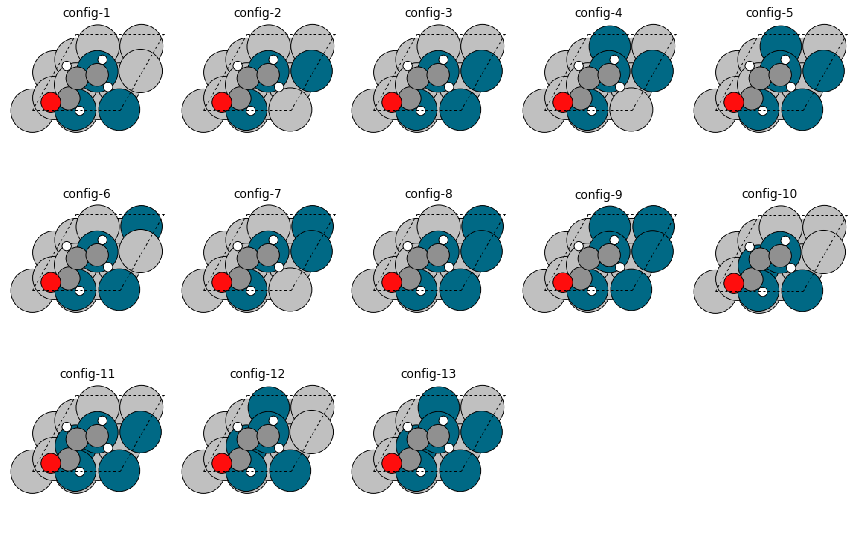
\includegraphics[width=.9\linewidth]{obipy-resources/488c510fd61eaf8a765856c1b3f36ad3-27044S6T.png}
\end{center}



\section{Code to access the datasets for reproducing the main figures in the manuscript}
\label{sec:org95dcfa5}

This section shows how the figures in the manuscript were generated.

\subsection{Acceleration of the geometry optimization for Acrolein/AgPd}
\label{sec:org44d385b}

\begin{minted}[frame=lines,fontsize=\scriptsize,linenos]{ipython}
from ase.io.trajectory import Trajectory
import numpy as np
from matplotlib import pyplot as plt
%matplotlib inline


single_steps = []
multi_steps = []
warm_steps = []
gpr_steps = []

for i in range(13):
    single_traj = Trajectory(f'./Acrolein-AgPd-single-multiple-configs/single-config-scratch-trajs/config-{i+1}.traj')
    single_steps.append(len(single_traj))
    multi_traj = Trajectory(f'./Acrolein-AgPd-single-multiple-configs/multi-config-scratch-trajs/config-{i+1}.traj')
    multi_steps.append(len(multi_traj))
    warm_traj = Trajectory(f'./Acrolein-AgPd-single-multiple-configs/multi-config-warmup-trajs/config-{i+1}.traj')
    warm_steps.append(len(warm_traj))
    gpr_traj = Trajectory(f'./Acrolein-AgPd-single-multiple-configs/gpr-trajs/config-{i+1}.traj')
    gpr_steps.append(len(gpr_traj))

steps = [single_steps, multi_steps, warm_steps, gpr_steps]
labels = ['single', 'multiple', 'warm up', 'GPR']
mean_labels = ['single mean', 'multiple mean', 'warm up mean', 'GPR_mean']
xs = range(1, 14)

f, (ax, ax2) = plt.subplots(2, 1, sharex=True, figsize=(8, 5), )
ax.plot(xs, steps[3], '-o', label = labels[3], color=f'C{3}')
means = [round(np.mean(steps[3]), 1)] * len(xs)
ax.plot(xs, means, '--', color=f'C{3}', label = mean_labels[3])
ax.text(1, means[0] + 0.4, str(means[0]))
ax.set_xticks(range(1, 14))

for i in range(3):
    ax2.plot(xs, steps[i], '-o', label = labels[i])
    means = [round(np.mean(steps[i]), 1)] * len(xs)
    ax2.plot(xs, means, '--', color=f'C{i}', label = mean_labels[i])
    ax2.text(1, means[0] + 0.4, str(means[0]))

ax2.set_xticks(range(1, 14))
ax.spines['bottom'].set_visible(False)
ax2.spines['top'].set_visible(False)
ax.xaxis.tick_top()
ax.tick_params(labeltop=False)
ax2.xaxis.tick_bottom()
d = .015
kwargs = dict(transform=ax.transAxes, color='k', clip_on=False)
ax.plot((-d, +d), (-d, +d), **kwargs) 
ax.plot((1 - d, 1 + d), (-d, +d), **kwargs)
kwargs.update(transform=ax2.transAxes)
ax2.plot((-d, +d), (1 - d, 1 + d), **kwargs)
ax2.plot((1 - d, 1 + d), (1 - d, 1 + d), **kwargs)

ax2.set_xlabel('configuration', fontsize=14)
ax2.set_ylabel('# of DFT calls', fontsize=14)
ax2.yaxis.set_label_coords(-0.07, 1.0)
f.legend(bbox_to_anchor=(0.12, 1.0), ncol=4, loc='upper left')
f.savefig('./single-multi-warmup-gpr.png', dpi=300)
\end{minted}

\begin{verbatim}
<Figure size 576x360 with 2 Axes>
\end{verbatim}


\begin{center}
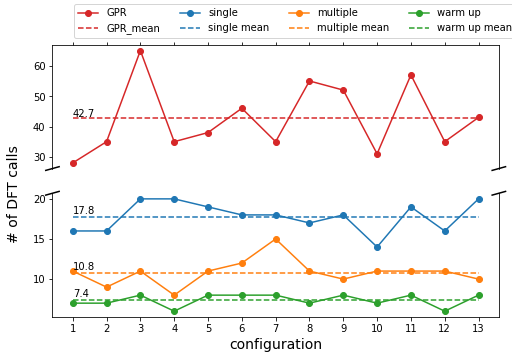
\includegraphics[width=.9\linewidth]{obipy-resources/488c510fd61eaf8a765856c1b3f36ad3-27044fEa.png}
\end{center}


\subsection{Performance for various systems}
\label{sec:org5312cd6}

\begin{minted}[frame=lines,fontsize=\scriptsize,linenos]{ipython}
from matplotlib import pyplot as plt
import pickle
import numpy as np

path = 'more-geometry-optimization-data'

with open(f'./{path}/AuPd-slab-vasp-data-25.pkl', 'rb') as f:
    slab_vasp_data = pickle.load(f)

with open(f'./{path}/AuPd-slab-nn-data-25.pkl', 'rb') as f:
    slab_nn_data = pickle.load(f)

with open(f'./{path}/Acrolein-AgPd-vasp-data-100.pkl', 'rb') as f:
    ads_vasp_data = pickle.load(f)

with open(f'./{path}/Acrolein-AgPd-nn-data-scratch-100.pkl', 'rb') as f:
    ads_nn_data = pickle.load(f)

with open(f'./{path}/CO-AuPd-Ico-vasp-data-10.pkl', 'rb') as f:
    nano_vasp_data = pickle.load(f)

with open(f'./{path}/CO-AuPd-Ico-nn-data-10.pkl', 'rb') as f:
    nano_nn_data = pickle.load(f)

ads_nn_step_mean = np.mean(ads_nn_data['steps'])
ads_vasp_step_mean = np.mean(ads_vasp_data['steps'])

slab_nn_step_mean = np.mean(slab_nn_data['steps'])
slab_vasp_step_mean = np.mean(slab_vasp_data['steps'])

nano_nn_step_mean = np.mean(nano_nn_data['steps'])
nano_vasp_step_mean = np.mean(nano_vasp_data['steps'])

step_mean = np.array([slab_nn_step_mean, slab_vasp_step_mean, nano_nn_step_mean,
                      nano_vasp_step_mean, ads_nn_step_mean, ads_vasp_step_mean])

nn_steps = step_mean[[0, 2, 4]]
vasp_steps = step_mean[[1, 3, 5]]
nn_xs = [1, 2.5, 4]
vasp_xs = [1.5, 3, 4.5]

fig = plt.figure(figsize=(7, 5))
ax = fig.add_subplot(111)
ax.bar(nn_xs, nn_steps, width=0.5, label='NN AL')
ax.bar(vasp_xs, vasp_steps, width=0.5, label='VASP QN')
ax.set_ylabel('DFT calls')
ax.set_yticks(range(0, 160, 20))
ax.set_xticks([1.25, 2.75, 4.25])
ax.set_xticklabels(['AuPd FCC111', 'CO/AuPd Icosahedron', 'Acrolein/AgPd FCC111'])
ax.legend(loc='upper left')
ax.text(0.95, 7.5, str(nn_steps[0]))
ax.text(1.35, vasp_steps[0] + 1.1, str(vasp_steps[0]))
ax.text(2.4, nn_steps[1] + 1.1, str(nn_steps[1]))
ax.text(2.9, vasp_steps[1] + 1.1, str(vasp_steps[1]))
ax.text(3.85, nn_steps[2] + 1.1, str(nn_steps[2]))
ax.text(4.3, vasp_steps[2] + 1.1, str(vasp_steps[2]))
\end{minted}

\begin{verbatim}
Text(4.3, 119.99, '118.89')
\end{verbatim}


\begin{verbatim}
<Figure size 504x360 with 1 Axes>
\end{verbatim}


\begin{center}
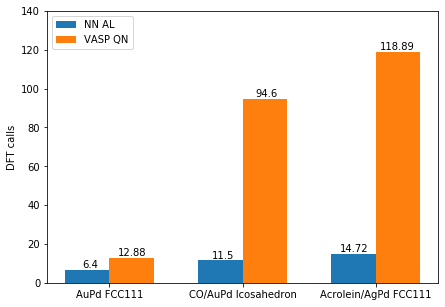
\includegraphics[width=.9\linewidth]{obipy-resources/488c510fd61eaf8a765856c1b3f36ad3-27044sOg.png}
\end{center}

\begin{minted}[frame=lines,fontsize=\scriptsize,linenos]{ipython}
from ase.db import connect
from matplotlib import pyplot as plt

init_db = connect('./Acetylele-hydrogenation-NEB/Acetylene-hydro-initial-configs.db')
vasp_db = connect('./Acetylele-hydrogenation-NEB/Acetylenen-hydro-vasp-cnvg.db')
nn_db = connect('./Acetylele-hydrogenation-NEB/Acetylene-hydro-nn-cnvg.db')

init_nrgs = [entry.energy for entry in init_db.select()]
vasp_nrgs = [entry.energy for entry in vasp_db.select()]
nn_nrgs = [entry.energy for entry in nn_db.select()]
xs = range(len(vasp_nrgs))

fig = plt.figure()
ax = fig.add_subplot(111)
ax.plot(xs, nn_nrgs, '-o')
ax.plot(xs, vasp_nrgs, '-o')
ax.set_xlabel('Reaction coordinate')
ax.set_ylabel('energy (eV)')
ax.legend(['NN ensemble', 'Vasp'])
vasp_act = vasp_nrgs[5] - vasp_nrgs[0]
nn_act = nn_nrgs[5] - nn_nrgs[0]
ax.text(3.5, -204.6, 'Activation energy:')
ax.text(3.5, -204.65, f'NN ensemble: {round(nn_act, 3)} eV')
ax.text(3.5, -204.7, f'Vasp: {round(vasp_act, 3)} eV')
\end{minted}

\begin{verbatim}
Text(3.5, -204.7, 'Vasp: 0.814 eV')
\end{verbatim}


\begin{verbatim}
<Figure size 432x288 with 1 Axes>
\end{verbatim}


\begin{center}
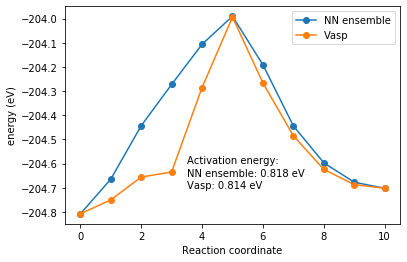
\includegraphics[width=.9\linewidth]{obipy-resources/488c510fd61eaf8a765856c1b3f36ad3-270445Ym.png}
\end{center}


\section{Gaussian Process Regression}
\label{sec:orgc135a39}
We adapt the Gaussian Process Regression (GRP) method from previous literatures \cite{torres-2019-low-scalin,koistinen-2017-nudged-elast} as one of the comparisons in this work. The GPR model uses the positions of the atoms as the feature \(\textbf{X} = [\textbf{x}_1, ..., \textbf{x}_N]\), and the model is trained on the corresponding energies (\(\textbf{e}\)) and the first order derivative which is the negative forces in this application. Thus,  \(\textbf{y} = [\textbf{e}, -\textbf{f}_1, ..., -\textbf{f}_N]\)

Therefore, the prediction function could be sampled from the Gaussian Process defined by a prior mean and a kernel function:

\begin{equation}
f(x) \sim \mathbb{GP}\left(\boldsymbol{\mu}, k\left( \boldsymbol{x}, \boldsymbol{x'} \right) \right)
\end{equation}

where \({\mu}\) is the prior for the energies and forces and it is set as zero in our work. Given a training set \(\mathbb{D}\), the predicted mean and variance are
\begin{equation}
\mathbb{E} \left[ f(\boldsymbol{x}| \mathbb{D})\right] = \boldsymbol{k}(\boldsymbol{x}) \left[ \boldsymbol{K} (\boldsymbol{x} + \sigma_{n}^2 \boldsymbol{I})\right]^{-1} \boldsymbol{y}
\end{equation}

and 

\begin{equation}
\mathbb{V} \left[ f(\boldsymbol{x}| \mathbb{D})\right] = k(\boldsymbol{x}, \boldsymbol{x}) -  \boldsymbol{k}(\boldsymbol{x})^{T} \left[ \boldsymbol{K} (\boldsymbol{x} + \sigma_{n}^2 \boldsymbol{I})\right]^{-1} \boldsymbol{k}(\boldsymbol{x})
\end{equation}

where \(\sigma_{n}\) is the noise of the data. 

The kernel function could be partitioned into:

\begin{equation}
\boldsymbol{K}(\boldsymbol{x}) = 
\begin{pmatrix}
\boldsymbol{K}_{ee}(\boldsymbol{x}, \boldsymbol{x}) & \boldsymbol{K}_{ef}(\boldsymbol{x}, \boldsymbol{x})  \\
\boldsymbol{K}_{ef}(\boldsymbol{x}, \boldsymbol{x}) & \boldsymbol{K}_{ff}(\boldsymbol{x}, \boldsymbol{x}) 
\end{pmatrix}

\end{equation}

Squared exponential kernel is used in our implementation. Thus, the formula for these kernel function are:

\begin{equation}
k_{ee}(\boldsymbol{x}, \boldsymbol{x'}) = \sigma _{f}^{2} \exp{\left( -\frac{1}{2}\sum_{d=1}^{D} \frac{(x_{d} - x_{d}')^2}{l_{d}^{2}}\right)}
\end{equation}


\begin{equation}
k_{fe}(\boldsymbol{x}, \boldsymbol{x'}) = -\frac{\sigma _{f}^{2}(x_{d} - x_{d}')}{l_{d}^{2}}} \exp{\left( -\frac{1}{2}\sum_{j=1}^{D} \frac{(x_{j} - x_{j}')^2}{l_{j}^{2}}\right)}
\end{equation}

\begin{equation}
k_{ff}(\boldsymbol{x}, \boldsymbol{x'}) =  \frac{-\sigma _{f}^{2}}{l_{d1}^{2}} \left( \delta_{d_{1}d_{2}} - \frac{(x_{d1} - x_{d1}')(x_{d2} - x_{d2}')}{l_{d1}^{2}}\right)  \exp{\left( -\frac{1}{2}\sum_{j=1}^{D} \frac{(x_{j} - x_{j}')^2}{l_{j}^{2}}\right)}
\end{equation}

where \(\sigma_{f}\) is fixed as 1.0, and the bandwidth \(l\) is optimized isotropically.

\bibliography{references}
\end{document}